% ============================================================
%  §3  Method
% ============================================================
\label{sec:method}

\begin{figure*}[t]
  \centering
  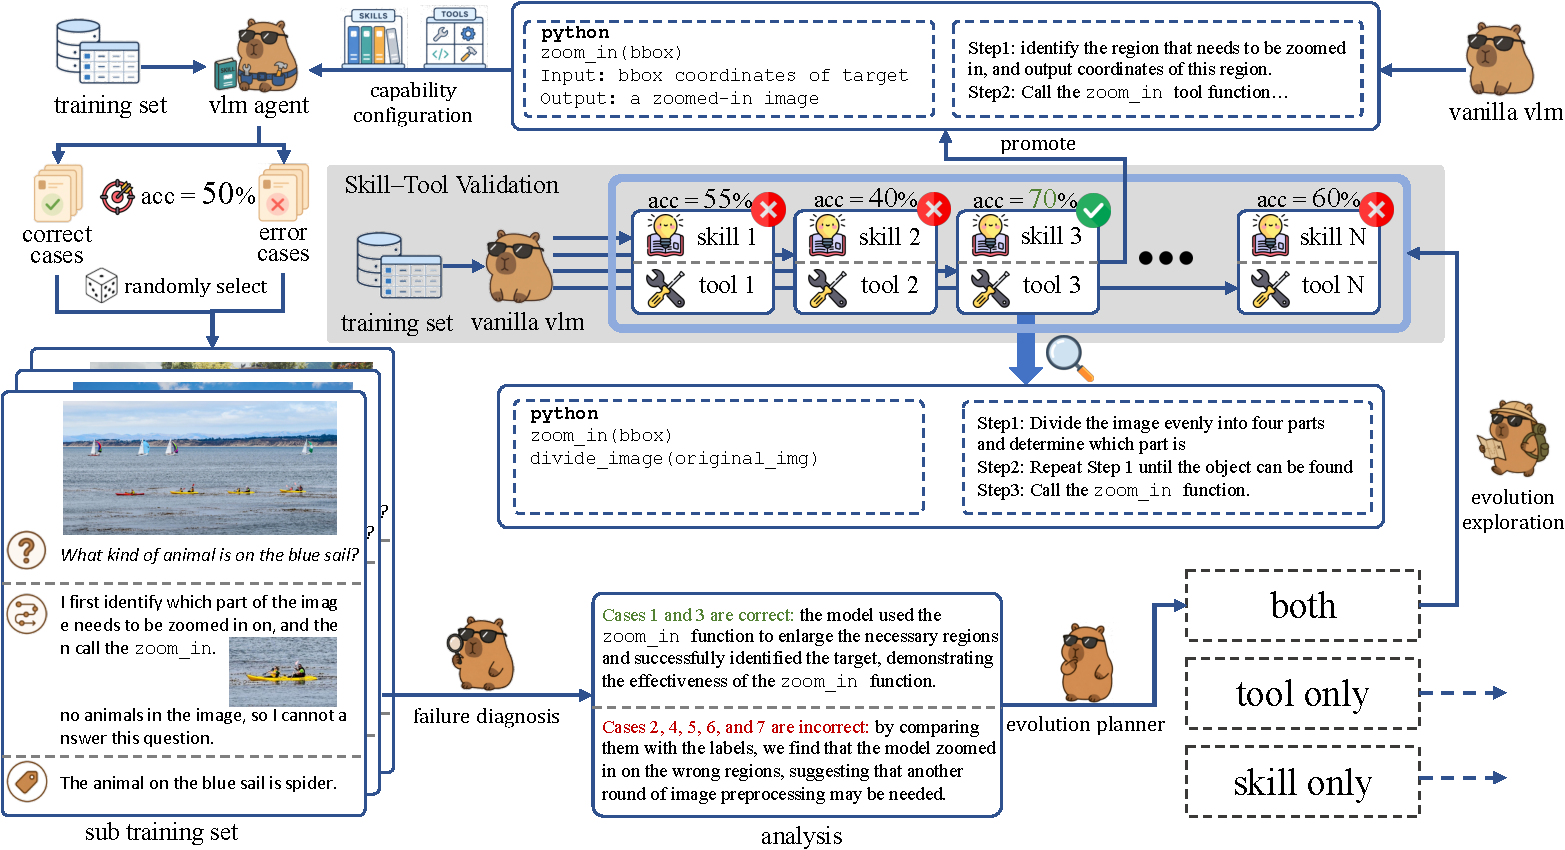
\includegraphics[width=\textwidth]{figures/method.pdf}
  \caption{
    \textbf{\sysname{} evolution loop.}
    On a sampled sub-training set, \sysname{} diagnoses both correct and incorrect attempts,
    explores candidate skill$+$tool capabilities, and promotes the best by validation into a
    persistent library.
  }
  \label{fig:method}
\end{figure*}

\subsection{Problem Formulation}
\label{sec:method_formulation}

Let $\mathcal{D}_{\text{train}} = \{(x_i, y_i, \mathbf{v}_i)\}_{i=1}^{k}$ denote a small training
subset of $k$ cases, where $x_i$ is the question, $y_i$ the ground-truth answer, and $\mathbf{v}_i$
the associated visual input (one or more images).
Let $\pi_\theta$ be a frozen VLM backbone (no gradient updates permitted).
We define a capability set $\mathcal{C} = \{\mathcal{S}, \mathcal{T}\}$, where
$\mathcal{S}$ is a library of \emph{skills} (structured reasoning SOPs) and
$\mathcal{T}$ is a library of \emph{tools} (executable Python programs).
An agent $f_{\mathcal{C}}$ operates by retrieving relevant capabilities from $\mathcal{C}$,
applying them during problem solving, and invoking $\pi_\theta$ for reasoning.
Our goal is to learn $\mathcal{C}$ from $\mathcal{D}_{\text{train}}$ to maximise performance on a
held-out validation set $\mathcal{D}_{\text{val}}$, subject to the constraint
$\nabla_\theta = 0$ (no weight updates).

\subsection{Evolution Loop}
\label{sec:method_loop}

Each evolution iteration over $\mathcal{D}_{\text{train}}$ has three phases
(Figure~\ref{fig:method}).

\textbf{Diagnose.}
The agent solves $\mathcal{D}_{\text{train}}$ with the current $\mathcal{C}$, then samples a
sub-training set $\mathcal{D}_{\text{sub}} \subseteq \mathcal{D}_{\text{train}}$ containing
both correct and incorrect attempts. The \textsc{AnalyzerDecider} inspects
$\mathcal{D}_{\text{sub}}$---the questions, original images $\mathbf{v}_i$, reasoning
traces $\tau_i$, and any intermediate tool outputs---and emits a root-cause analysis grounded
in visual evidence, an identified bottleneck type (\emph{cognitive} when the visual evidence
is available but the reasoning procedure is weak, or \emph{perceptual} when the agent needs a
transformed visual input), and an action $a \in \{\texttt{skill}, \texttt{tool}, \texttt{both}\}$.
Visual input here is essential: deciding whether a crop is misaligned, whether labels are
legible, or whether a processed image introduced artefacts requires inspecting the image, not
just the reasoning trace.

\textbf{Explore.}
Conditioned on the diagnosis, the \textsc{Generator} proposes $M$ candidate skill$+$tool
combinations, each addressing the diagnosed bottleneck with a different strategy or
implementation.

\textbf{Validate and promote.}
Each candidate is evaluated on $\mathcal{D}_{\text{train}}$, and the combination with the
highest accuracy is added to $\mathcal{C}$. Selection by accuracy on
$\mathcal{D}_{\text{train}}$ subsumes both an \emph{origin} requirement (the new capability
must improve over the previous $f_{\mathcal{C}}$ on the cases it targets) and a
\emph{regression} requirement (it must not degrade currently-correct cases). Promoted tools
then go through a mastery phase (Section~\ref{sec:method_tool}) that profiles when each tool
helps before exposing it at inference. The full procedure runs for $N$ iterations (default
$N{=}3$); pseudocode is given in Appendix~\ref{app:impl} (Algorithm~\ref{alg:main}).

\subsection{Skills}
\label{sec:method_skill}

A \emph{skill} is a structured Markdown document with four fields:
\textbf{When-to-Use} (a trigger predicate over question and image type),
\textbf{Strategy} (a numbered step-by-step SOP),
\textbf{Common Pitfalls}, and
\textbf{Worked Example}.
The Generator writes a skill conditioned on the AnalyzerDecider's root-cause analysis; if a
skill covering the same problem class already exists in $\mathcal{S}$, new insights are merged
into it rather than creating a duplicate, preventing library bloat. At inference, the Solver
retrieves the top-$K$ skills by BM25 similarity to the question and appends them to the system
prompt.

\subsection{Tools and Mastery}
\label{sec:method_tool}
\label{sec:method_mastery}

A \emph{tool} is a Python function ($\leq$150 lines) that takes one or more image paths and
returns processed images or extracted data, using standard CV libraries (OpenCV, PIL, NumPy).
The Generator writes a tool conditioned on a perceptual bottleneck diagnosis; representative
examples produced in our experiments include chart re-rendering with enlarged axis labels,
saliency-guided sub-region extraction, and contrast enhancement for low-quality documents.

\paragraph{Mastery profiling.}
For each promoted tool, \sysname{} runs a mastery phase: the tool is applied to a held-out set
of 50 similar cases sampled from $\mathcal{D}_{\text{train}}$, and the agent records per case
whether the tool improved, degraded, or had no effect on the final answer. From this profile,
the agent synthesises a \emph{mastery SOP}---a Markdown document describing the tool's
supported input patterns, negative patterns, and trigger conditions. The mastery SOP is
stored with the tool and consulted at inference to decide whether to invoke it, reducing
false-positive applications that would add latency or visual artefacts. This selective
invocation distinguishes \sysname{} from prior tool-creation
methods~\citep{tang2023creator, cai2024latm} that deploy generated tools indiscriminately.

\subsection{Tool Mastery from External Tool Sets (Mode B)}
\label{sec:method_mastery_ext}

The loop above (\textbf{Mode A}) both \emph{generates} tools and \emph{profiles} their
applicability. When a curated tool set $\mathcal{T}_0 \neq \emptyset$ is already provided,
\sysname{} can operate in \textbf{Mode B}: skip tool generation and apply the mastery
procedure directly to each $t_j \in \mathcal{T}_0$. Skill evolution proceeds unchanged.
Mode B requires no code generation and fewer LLM calls (one mastery profiling pass per tool),
making it practical when tool quality is already high but deployment strategy is unknown.
Experiment~II (Section~\ref{sec:exp2}) evaluates this mode.
